\documentclass[letterpaper]{article}
\usepackage{amssymb}
\usepackage{fullpage}
\usepackage{changepage}
\usepackage{amsmath}
\usepackage{epsfig,float,alltt}
\usepackage{psfrag,xr}
\usepackage[T1]{fontenc}
\usepackage{url}
\usepackage{pdfpages}
\usepackage{epstopdf}
\usepackage[framed,numbered,autolinebreaks,useliterate]{mcode}

%\includepdfset{pagecommand=\thispagestyle{fancy}}
\author{Fan Bu, Feng Zhou, Yi Yang}
\title{ME 552 Lab 01 Report}

\begin{document}
\date{09/17/2016}
\maketitle

\newcommand{\trace}{\mathrm{trace}}
\newcommand{\real}{\mathbb R}  % real numbers  {I\!\!R}
\newcommand{\nat}{\mathbb N}   % Natural numbers {I\!\!N}
\newcommand{\cp}{\mathbb C}    % complex numbers  {I\!\!\!\!C}
\newcommand{\ds}{\displaystyle}
\newcommand{\mf}[2]{\frac{\ds #1}{\ds #2}}
\newcommand{\spanof}[1]{\textrm{span} \{ #1 \}}
\newcommand{\sol}[0]{\textbf{Solution: }}
\newcommand{\pf}[0]{\textbf{Proof:}}
\newcommand{\rme}[0]{\textrm{e}}
\newcommand{\Null}[1]{\textrm{Null}\{#1\}}
\parindent 0pt
%%%%%%%%%%%%%%%%%%%%%%%%%%%%%%%%%%%%%%%%%%%%%%%%%%%%%%%%%%%%%%%%%%%%%%%%%%%%%%%
% Solution for Question 1 begins here - by Yi Yang
%%%%%%%%%%%%%%%%%%%%%%%%%%%%%%%%%%%%%%%%%%%%%%%%%%%%%%%%%%%%%%%%%%%%%%%%%%%%%%%
\section*{Question 1}
\subsection*{(a)}
We design the circuit as shown below:\\
\begin{figure}[h]
\begin{center}
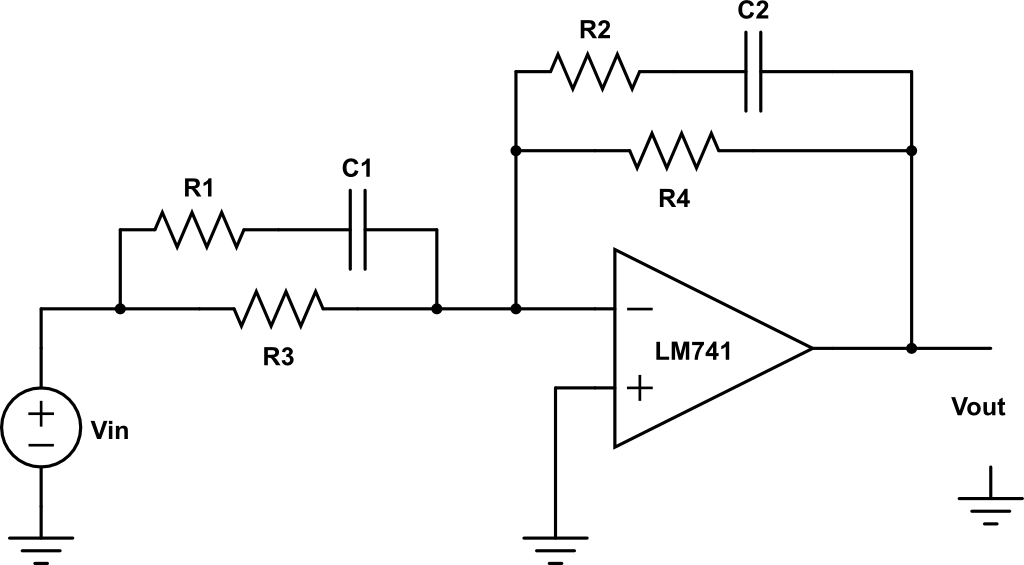
\includegraphics[width=10cm]{q1_circuitDiagram.png}
\end{center}
\caption{A lead-lag compensator circuit diagram for question 1.}
\label{q1_a}
\end{figure}
\subsection*{(b)}
We can let $R_1$, $C_1$, $R_3$ and $R_2$, $C_2$, $R_4$ form two different impedance module separately, and let their impedance equal $Z_1$ and $Z_2$, we can get:
$$Z_1 = \frac{R_3 * (R_1 + (1/sC_1))}{R_3 + (R_1 + (1/sC_1))} = \frac{R_3(sR_1C_1 +1)}{s(R_1C_1 + R_3C_1) + 1}$$
$$Z_2 = \frac{R_4 * (R_2 + (1/sC_2))}{R_4 + (R_2 + (1/sC_2))} = \frac{R_4(sR_2C_2 +1)}{s(R_2C_2 + R_4C_2) + 1}$$
The new circuits can be seen as an inverting amplifier:
$$\frac{V_{out}(s)}{V_{in}(s)} = - \frac{Z_2}{Z_1} = -  \frac{R_4(sR_2C_2 +1)}{(s(R_2C_2 + R_4C_2) + 1)}\frac{(s(R_1C_1 + R_3C_1) + 1)}{R_3(sR_1C_1 +1)} $$
$$=  -  \frac{R_4}{R_3}\frac{(sR_2C_2 +1)}{(s(R_2C_2 + R_4C_2) + 1)}\frac{(s(R_1C_1 + R_3C_1) + 1)}{(sR_1C_1 +1)} $$
If we assume $R_3 = R_4$, we will gain the standard formula of lead-lag compensator.
$$ - \frac{(sR_2C_2 +1)}{(s(R_2C_2 + R_4C_2) + 1)}\frac{(s(R_1C_1 + R_3C_1) + 1)}{(sR_1C_1 +1)}  = \frac{(1+0.1s)(1 + 5s)}{(1+0.01s)(1 + 10s)}$$
As illustrated in Lab1 instruction file, we can use two methods to invert the output polarity, so we could directly get the following equations:
$$R_1C_1 = 0.01$$
$$R_2C_2 = 5$$
$$R_1C_1 + R_3C_1 = 0.01 + R_3C_1 = 0.1$$
$$\implies R_3C_1 = 0.09$$
$$R_2C_2 + R_4C_2 = 5 + R_4C_2 = 10$$
$$\implies R_4C_2 = 5$$
$$\therefore R_4 = R_2 = R_3$$
\subsection*{(c)}
While building this circuit, we made the following assumptions:
\begin{itemize}
\item The op-amps we use are ideal, i.e. the input impedance is infinite and the output impedance is negligible. This implies that the op-amp does not load it's input circuit and loading effects are not seen on the op-amps output terminal.

\item The voltage at the inverting terminal is equal to the voltage at the non-inverting terminal.

\item The open loop op-amp gain is infinite.

\item The op-amp will operate in an ideal manner when the output is not saturated above or below its supply limits.

\item We assumed that the performance of the system is not overly sensitive to variations in resistance and we assumed the values of that the resistors were accurate and that capacitors had negligible internal resistance.
\end{itemize}
\subsection*{(d)}
We can set values to capacitors and resistors arbitrarily. However, the values we can choose for resistors are more flexible than capacitors. Thus, we decide to set the appropriate values to capacitors first and then determine the values of resistors. According to the formulas in section (b), we can choose values as shown below:
\begin{table}[H]
\begin{center}
    \begin{tabular}{|c|c|c|}
        \hline
        \textbf{Component Name} & \textbf{Component Type} & \textbf{Component Specification} \\ \hline
       $ LM 741$                     & \text{Signal Op-amp}         & $ \ V+ = +15V, V- = -15V     $             \\	
       $ C_1$                     & \text{Electrolytic Capacitor}         & $ \ 1 \mu F     $             \\ 
       $ C_2 $                   & \text{Electrolytic Capacitor}         & $ \ 55.55 \mu F     $               \\ 
       $ R_1  $                  & \text{Resistor}         & $ \ 10 K\Omega            $        \\ 
       $ R_2 $                    & \text{Resistor}         & $ \ 90 K\Omega        $            \\        
       $ R_3 $                   & \text{Resistor}         & $\ 90 K\Omega   $                 \\ 
       $ R_4$                     & \text{Resistor}         &$ \ 90 K\Omega$                    \\
        \hline
    \end{tabular}

\caption{Capacitances and Resistances chosen to construct the lead-lag controller}
\label{q1_td}
\end{center}
\end{table}
Having decided on the resistors, capacitors and op-amp that we need, we need further decide the voltage ratings for capacitors and wattage ratings for resistor, the wattage ratings should exceed the power supply of the system to ensure the safety of circuit components.
\subsection*{(e)}
Refer to the "Lab 1 Instructions" document and construct the circuits and collect relevant data.
\subsection*{(f)}
Two Bode plots that include magnitude and phase for the above transfer function is listed below:
\begin{figure}[H]
	\centering
	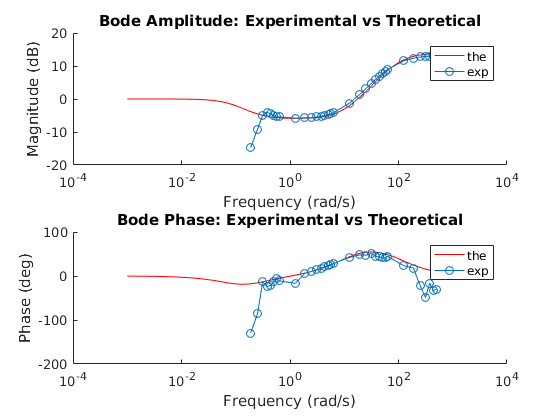
\includegraphics[scale=1.0]{q1f_bode.png}
	\caption{Theoretical vs Experimental Bode Plot}
	\label{bode}
\end{figure}
\subsection*{(g)}
We see our experimental plots and theoretical plots are similar in a large range of frequency points. However, we also get experimental results highly deviated from the theoretical predictions at low frequency and high frequency. We suspect that the discrepancy at low frequency arising from the low measuring period and we can not get the full information of the low frequency output signal in a small measuring time horizon. At high frequency, we also see the deviation from the nominal curve and we think this phenomenon stems from the aliasing error of our DAQ system, according to Shannon-Nyquist Sampling Theorem, if the sampling rate is less than twice of the signal bandwidth, the reconstructed signal will be corrupted. Hence, for the high frequency signal, out DAQ system may have no adequate sampling rates to reconstruct it.
\subsection*{(h)}
The following table shows the maximum and minimum phase angles present in the bode plot of the actual and theoretical systems. We will omit results of frequency higher than $100 Hz$. 
\begin{table}[hbt]
\begin{center}
	\begin{tabular}{|c|c|c|}
		\hline
		 & \textbf{Theoretical System} & \textbf{Actual System}  \\ \hline
		Minimum Phase Angle (degrees) & -18.7562 &  -129.5890\\
		Minimum Phase Frequency (rads/s) & 0.1360 & 0.1885\\
		Maximum Phase Angle (degrees) & 54.7226 & 51.3608 \\ 
		Maximum Phase Frequency (rads/s) & 31.8346 &  31.4159\\ \hline
	\end{tabular}
\caption{Maximum and Minimum Phase Angles and Frequencies for Theoretical and Actual System}
\label{q1_th}
\end{center}
\end{table}

When we analyse the data and find the trends of lead-lag bode plot: at low frequency, when it represents as phase lead compensator accompanied with magnitude decreasing. However, at high frequency, when it represents as phase lag compensator accompanied with magnitude increasing.
\subsection*{(i)}
We can predict that the theoretical gain ratio at $1 Hz$ should approximately be $0.5896$ and at $100 Hz$ be $4.9385$, this is determined by the transfer function and independent of what amplitude of input signal we apply to the system. We need to confirm this through experiments, we have listed all the necessary values to the following table:
\begin{table}[hbt]
\begin{center}
    \begin{tabular}{|c|c|c|c|}
        \hline
        Input Frequency (Hz) & Input Amplitude (V) & Output Phase (degrees) & Output Gain \\ \hline
        1                    & 0.5             & 27.263973                & 0.60674               \\ 
        1                    & 1               & 28.872286                & 0.618304               \\ 
        1                    & 2               & 29.66062                & 0.6284775               \\ 
        100                  & 0.5             & -70.917477               & 4.476976                \\ 
        100                  & 1               & -15.294401               & 4.486602                \\ 
        100                  & 2               & 5.858839               & 4.4332675               \\
        \hline
    \end{tabular}
\end{center}
\caption{Amplitude dependence of system response at two different frequencies}
\label{q1_it}
\end{table}
The data listed on the table shows that our op-amp do not get saturated both under $1 Hz$ and $100 Hz$, and we also found the output gain for is approximately equal to the theoretical values. Hence, we can conclude that our circuit is correct.
\subsection*{(j)}
The Matlab codes used for generating Bode plots is attached:
\lstinputlisting[firstline=1, lastline=100]{question1.m}
The front panel and the block diagram of the Labview program is attached below:
\begin{figure}[H]
	\centering
	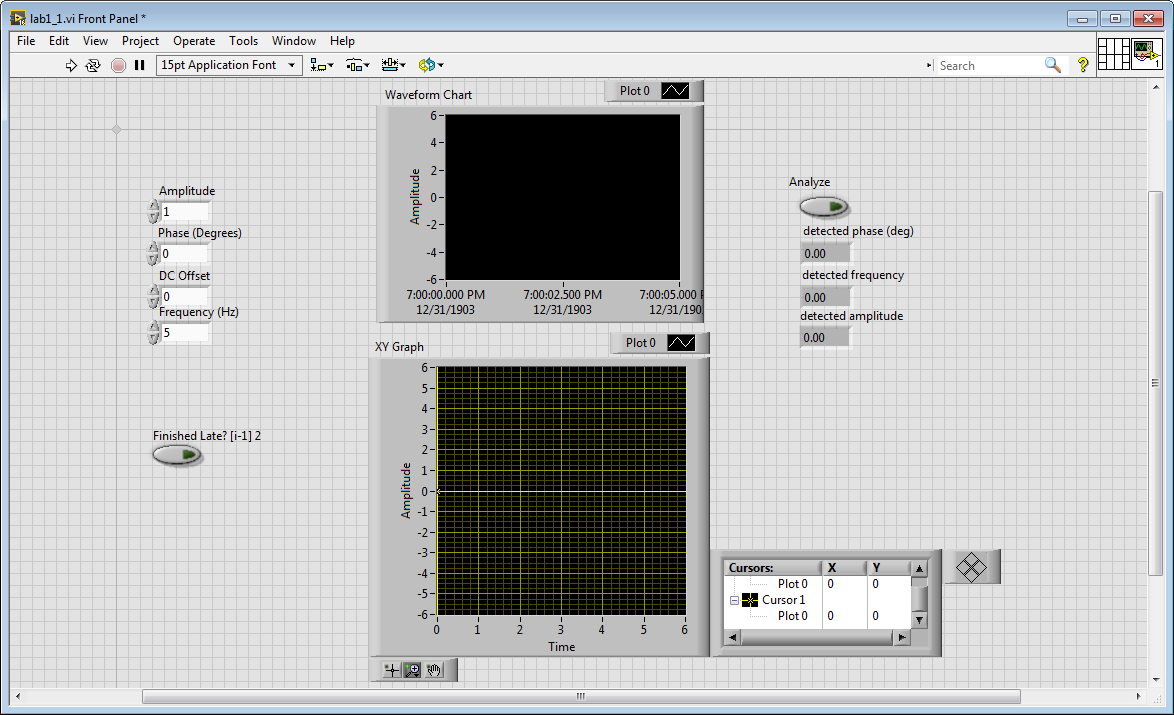
\includegraphics[scale=0.3]{front_panel.PNG}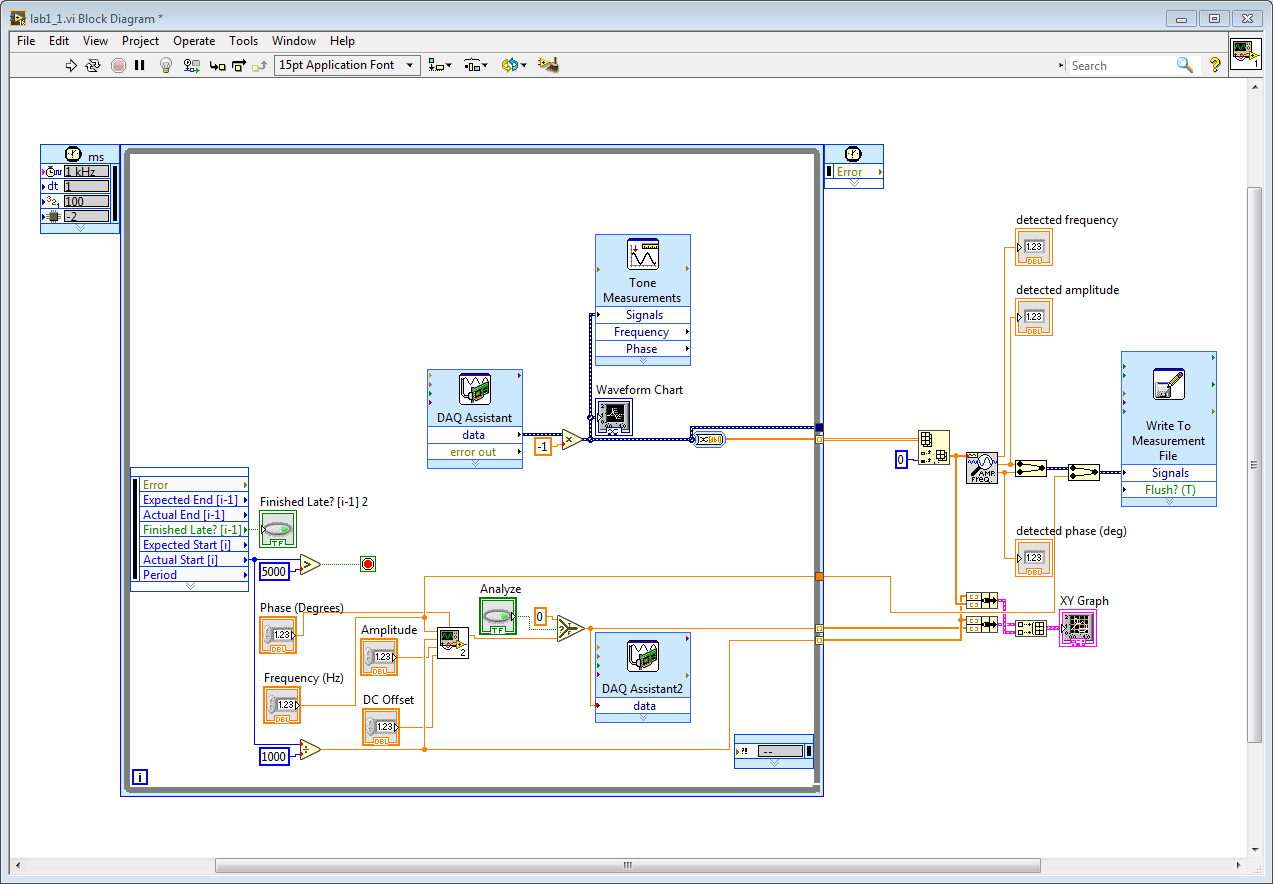
\includegraphics[scale=0.25]{block_diagram.PNG}
	\caption{Front Panel and Block Diagram of Labview program}
	\label{Fp_Bd}
\end{figure}
\section*{Qustion 2}
\subsection*{(a)}
The circuit diagram is listed below:
\begin{figure}[H]
	\centering
	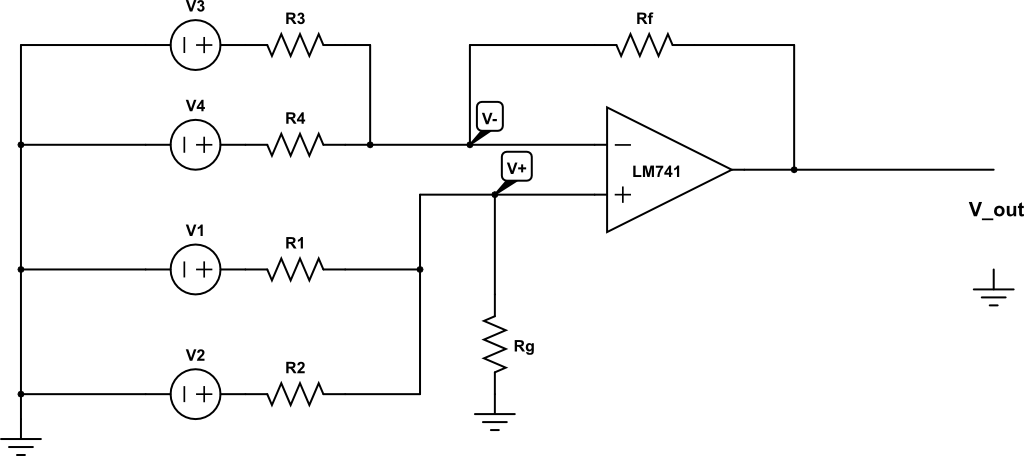
\includegraphics[width=13cm]{q2_circuitDiagram.png}
	\caption{Schematic of the Electrical Circuit}
	\label{fig:circuit2}
\end{figure}

\hspace*{3em}
\subsection*{(b)}
For this circuit, we can apply KVL and KCL to get the following equations:
$$\mf{V_3 - V_-}{R_3} + \mf{V_4 - V_-}{R_4} = \mf{V_- - V_{out}}{R_f}$$
$$\mf{V_1 - V_+}{R_1} + \mf{V_2 - V_+}{R_2} = \mf{V_+}{R_g}$$
$$V_- = V_+$$
Hence, we can get the following relations:
$$V_{out} = \mf{R_1//R_2//R_g}{R_3//R_4//R_f}\cdot\mf{R_6}{R_1}V_1 + \mf{R_1//R_2//R_g}{R_3//R_4//R_f}\cdot\mf{R_f}{R_2}V_2 - \mf{R_6}{R_3}V_3 -\mf{R_f}{R_4}V_4$$
$$V_{out} = V_1 + 2V_2 - 3V_3 -4V_4$$
Compare these two equations and we can get:
$$R_f = 4R_4,\; R_f = 3R_3,\; R_1 = 2R_2,\; R_2 = \mf{5}{2}R_g$$
\subsection*{(c)}
\begin{itemize}
	\item The op-amps gain $A_{o1}$ is infinite.
	\item $Z_{in}$ (input impedance) is infinite, so no current at input terminal
	\item $Z_{out}$ (output impedance) is zero, so $V_{out} = A_{o1}V_{in}$
	\item The time response is instantaneous
	\item The output voltage has a range because it can never be out of $[-V,\; +V]$
\end{itemize}
\subsection*{(d)}
We should consider Wattage ratings of circuit components to the circuit power supply to determine the values of circuit components. We can select one group of values arbitrarily and check the data sheet to promise that the wattage ratings exceed the circuit power supply. The values we chose for our circuit is listed on the following table:
\begin{table}[h]
\begin{center}
    \begin{tabular}{|c|c|c|}
        \hline
        \textbf{Component Name} & \textbf{Component Type} & \textbf{Component Specification} \\ \hline
	$ LM 741$                     & \text{Signal Op-amp}         & $ \ V+ = +15V, V- = -15V     $             \\	
       	$ R_f  $                  & \text{Resistor}         & $120 \ K\Omega            $        \\ 
	$ R_g $                    & \text{Resistor}         & $40 \ K\Omega        $            \\ 
       $ R_1$                     & \text{Resistor}         & $200 \ K\Omega        $             \\ 
       $ R_2 $                   & \text{Resistor}         & $100 \ K\Omega     $               \\ 
       $ R_3 $                   & \text{Resistor}         & $40 \ K\Omega   $                 \\ 
       $ R_4$                     & \text{Resistor}         &$ 30 \ K\Omega$                    \\
        \hline
    \end{tabular}
\end{center}
\label{q2_tabD}
\caption{Capacitances and Resistances to construct the summation circuit}
\end{table}
\subsection*{(e)}
Refer to the "Lab 1 Instruction" document to build the above circuit and collect relevant data.
\subsection*{(f)}
The screen shots for set $1$, $2$ and $3$ are listed below:
\begin{figure}[H]
	\centering
	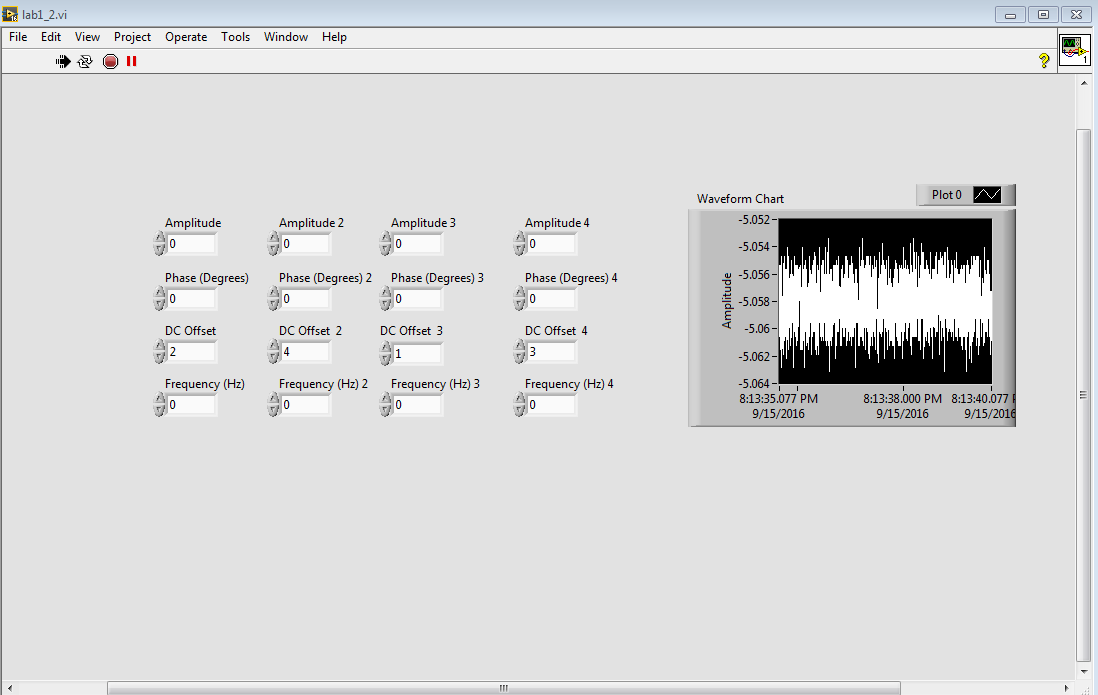
\includegraphics[scale=0.4]{f_set1.PNG}
	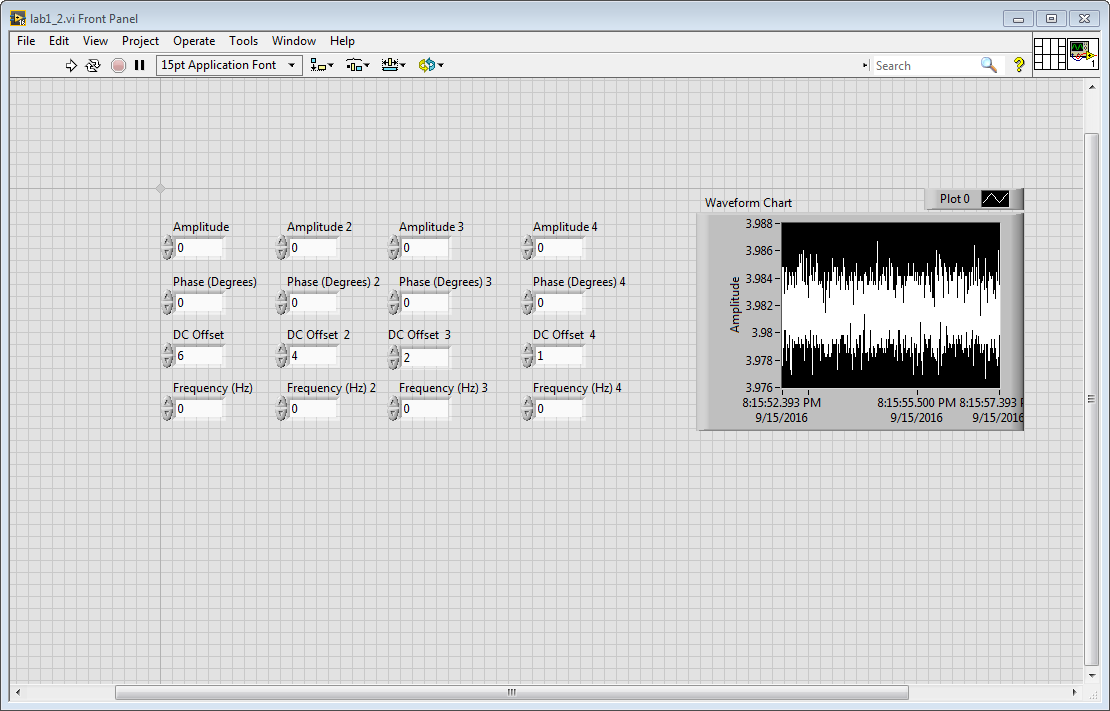
\includegraphics[scale=0.4]{f_set2.PNG}
	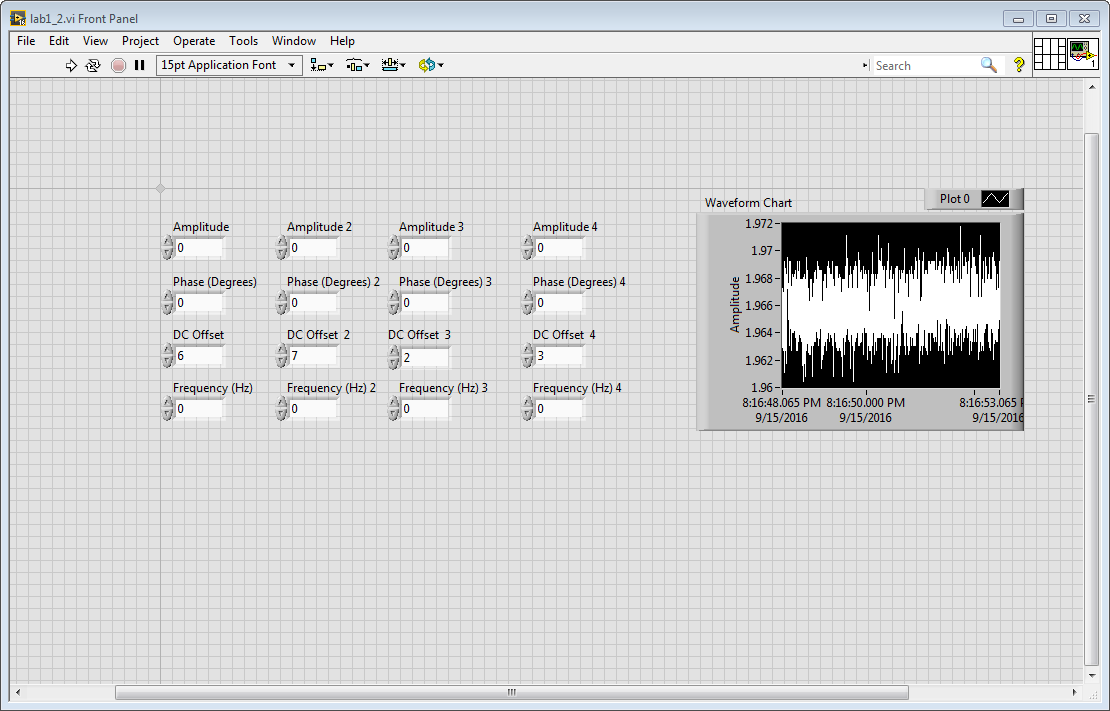
\includegraphics[scale=0.4]{f_set3.PNG}
	\caption{Labview Output Screen Shot for 3 Sets of Inputs}
	\label{fig:sc}
\end{figure}
\subsection*{(g)}
Feed 2 sets of input voltages into the voltage summer one by one and measure the output of the circuit. The Labview screen shot is listed below:
\begin{figure}[H]
	\centering
	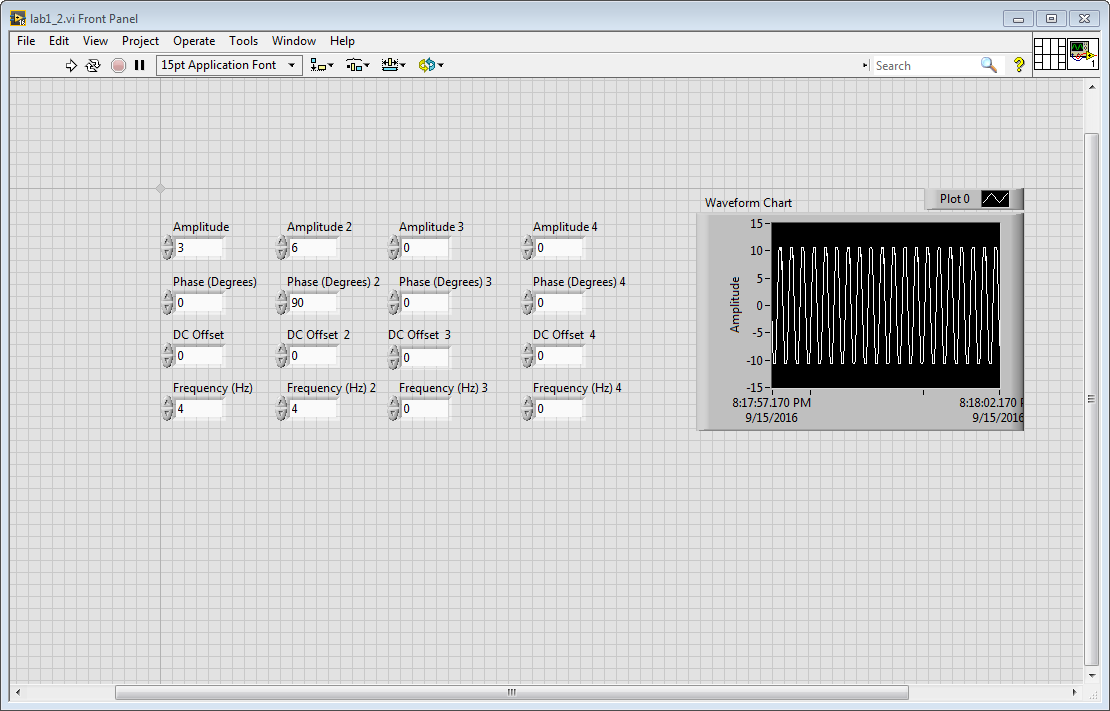
\includegraphics[scale=0.4]{g_set1.PNG}
	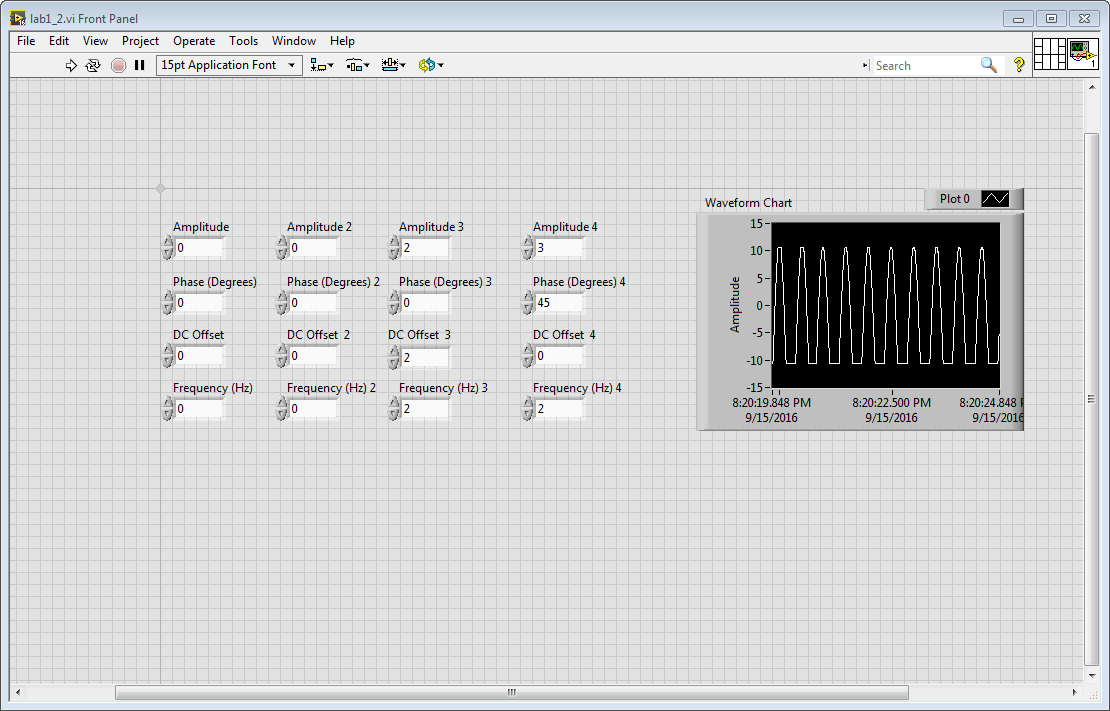
\includegraphics[scale=0.4]{g_set2.PNG}
	\caption{Labview Output Screen Shot for 2 Sets of Inputs}
	\label{fig:scs}
\end{figure}
We see when we input those two sets of AC signal, we will get the outputs as shown in the figure. We suppose the reason why both of two curves get saturated approximately at $\pm 11 V$ is not arisen from op-amp, as we see from the data sheet of Op-Amp, the saturated point for Op-Amp is within $2 V$ of the ideal Op-Amp power supply, which is greater than $11 V$, so the reason why we see a saturated phenomenon is out of DAQ system. From the data sheet of  NI 6230, we found that  NI 6230 DAQ card will limit the range of input signal to $\pm 10 V$, which is approximate to saturation point of the results shown in the Labview. We further use oscilloscope to measure the output signal to get the following results:
\begin{figure}[H]
	\centering
	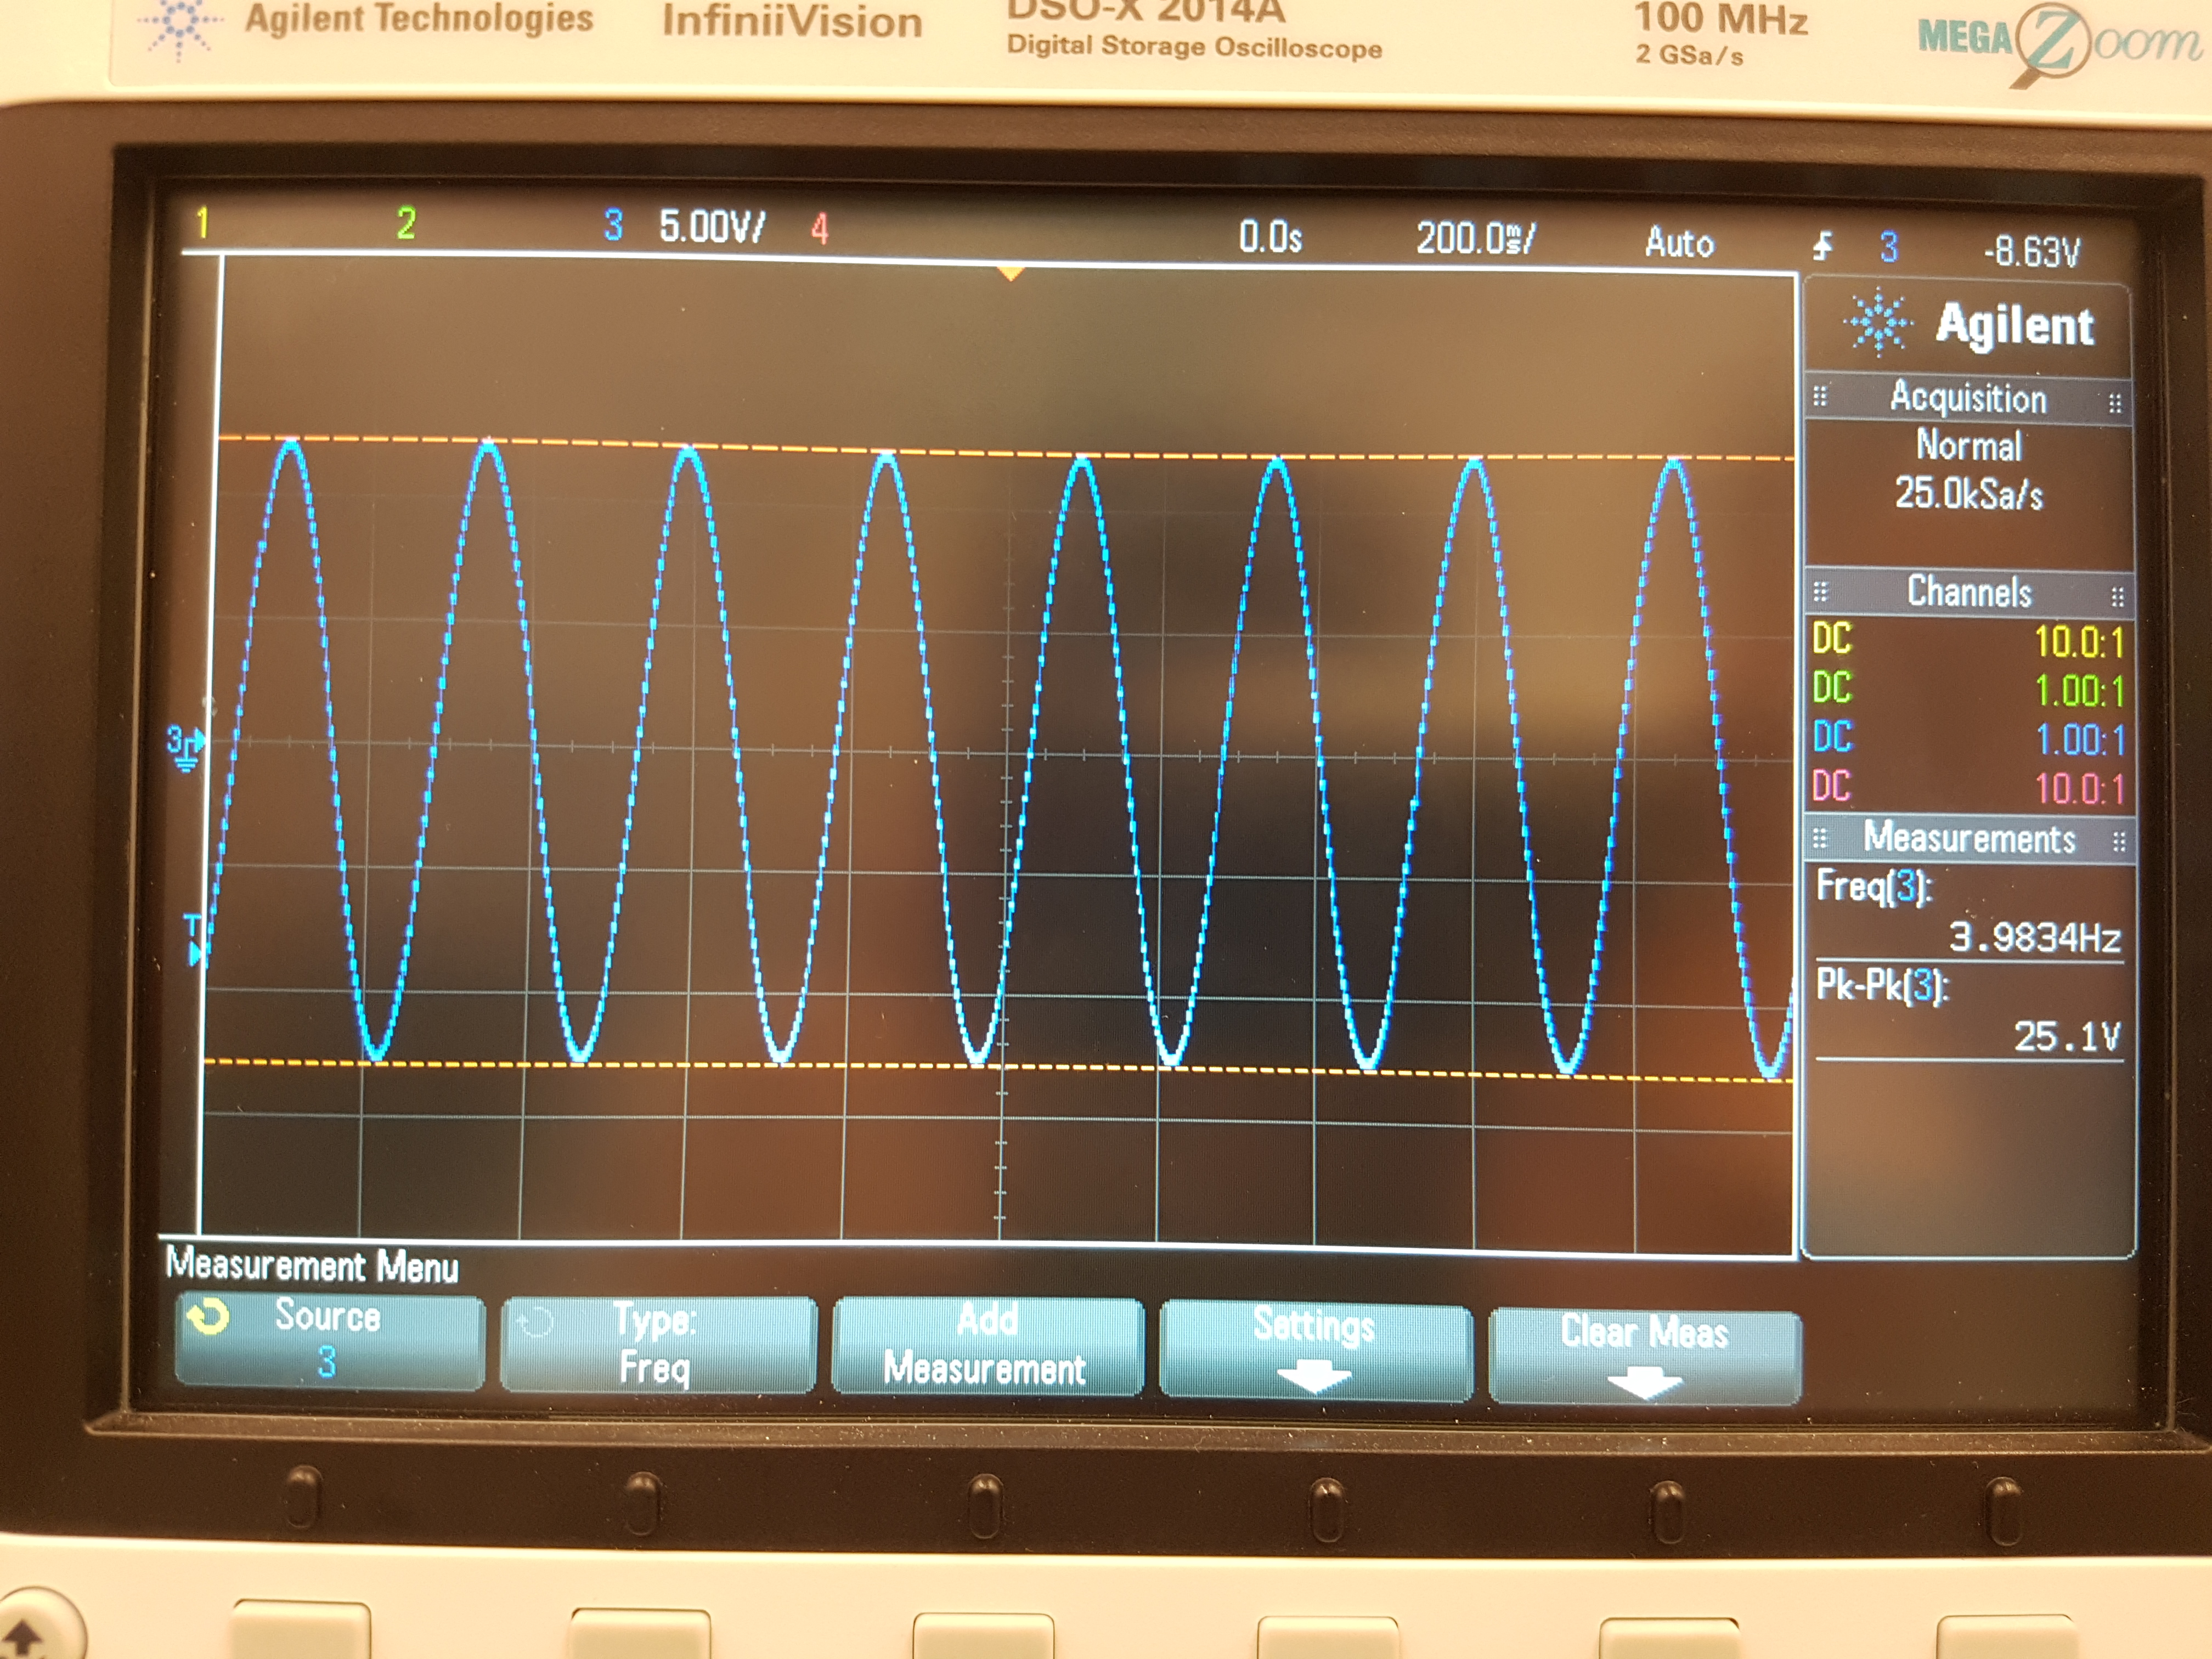
\includegraphics[scale=0.1]{osc_set1.jpg}
	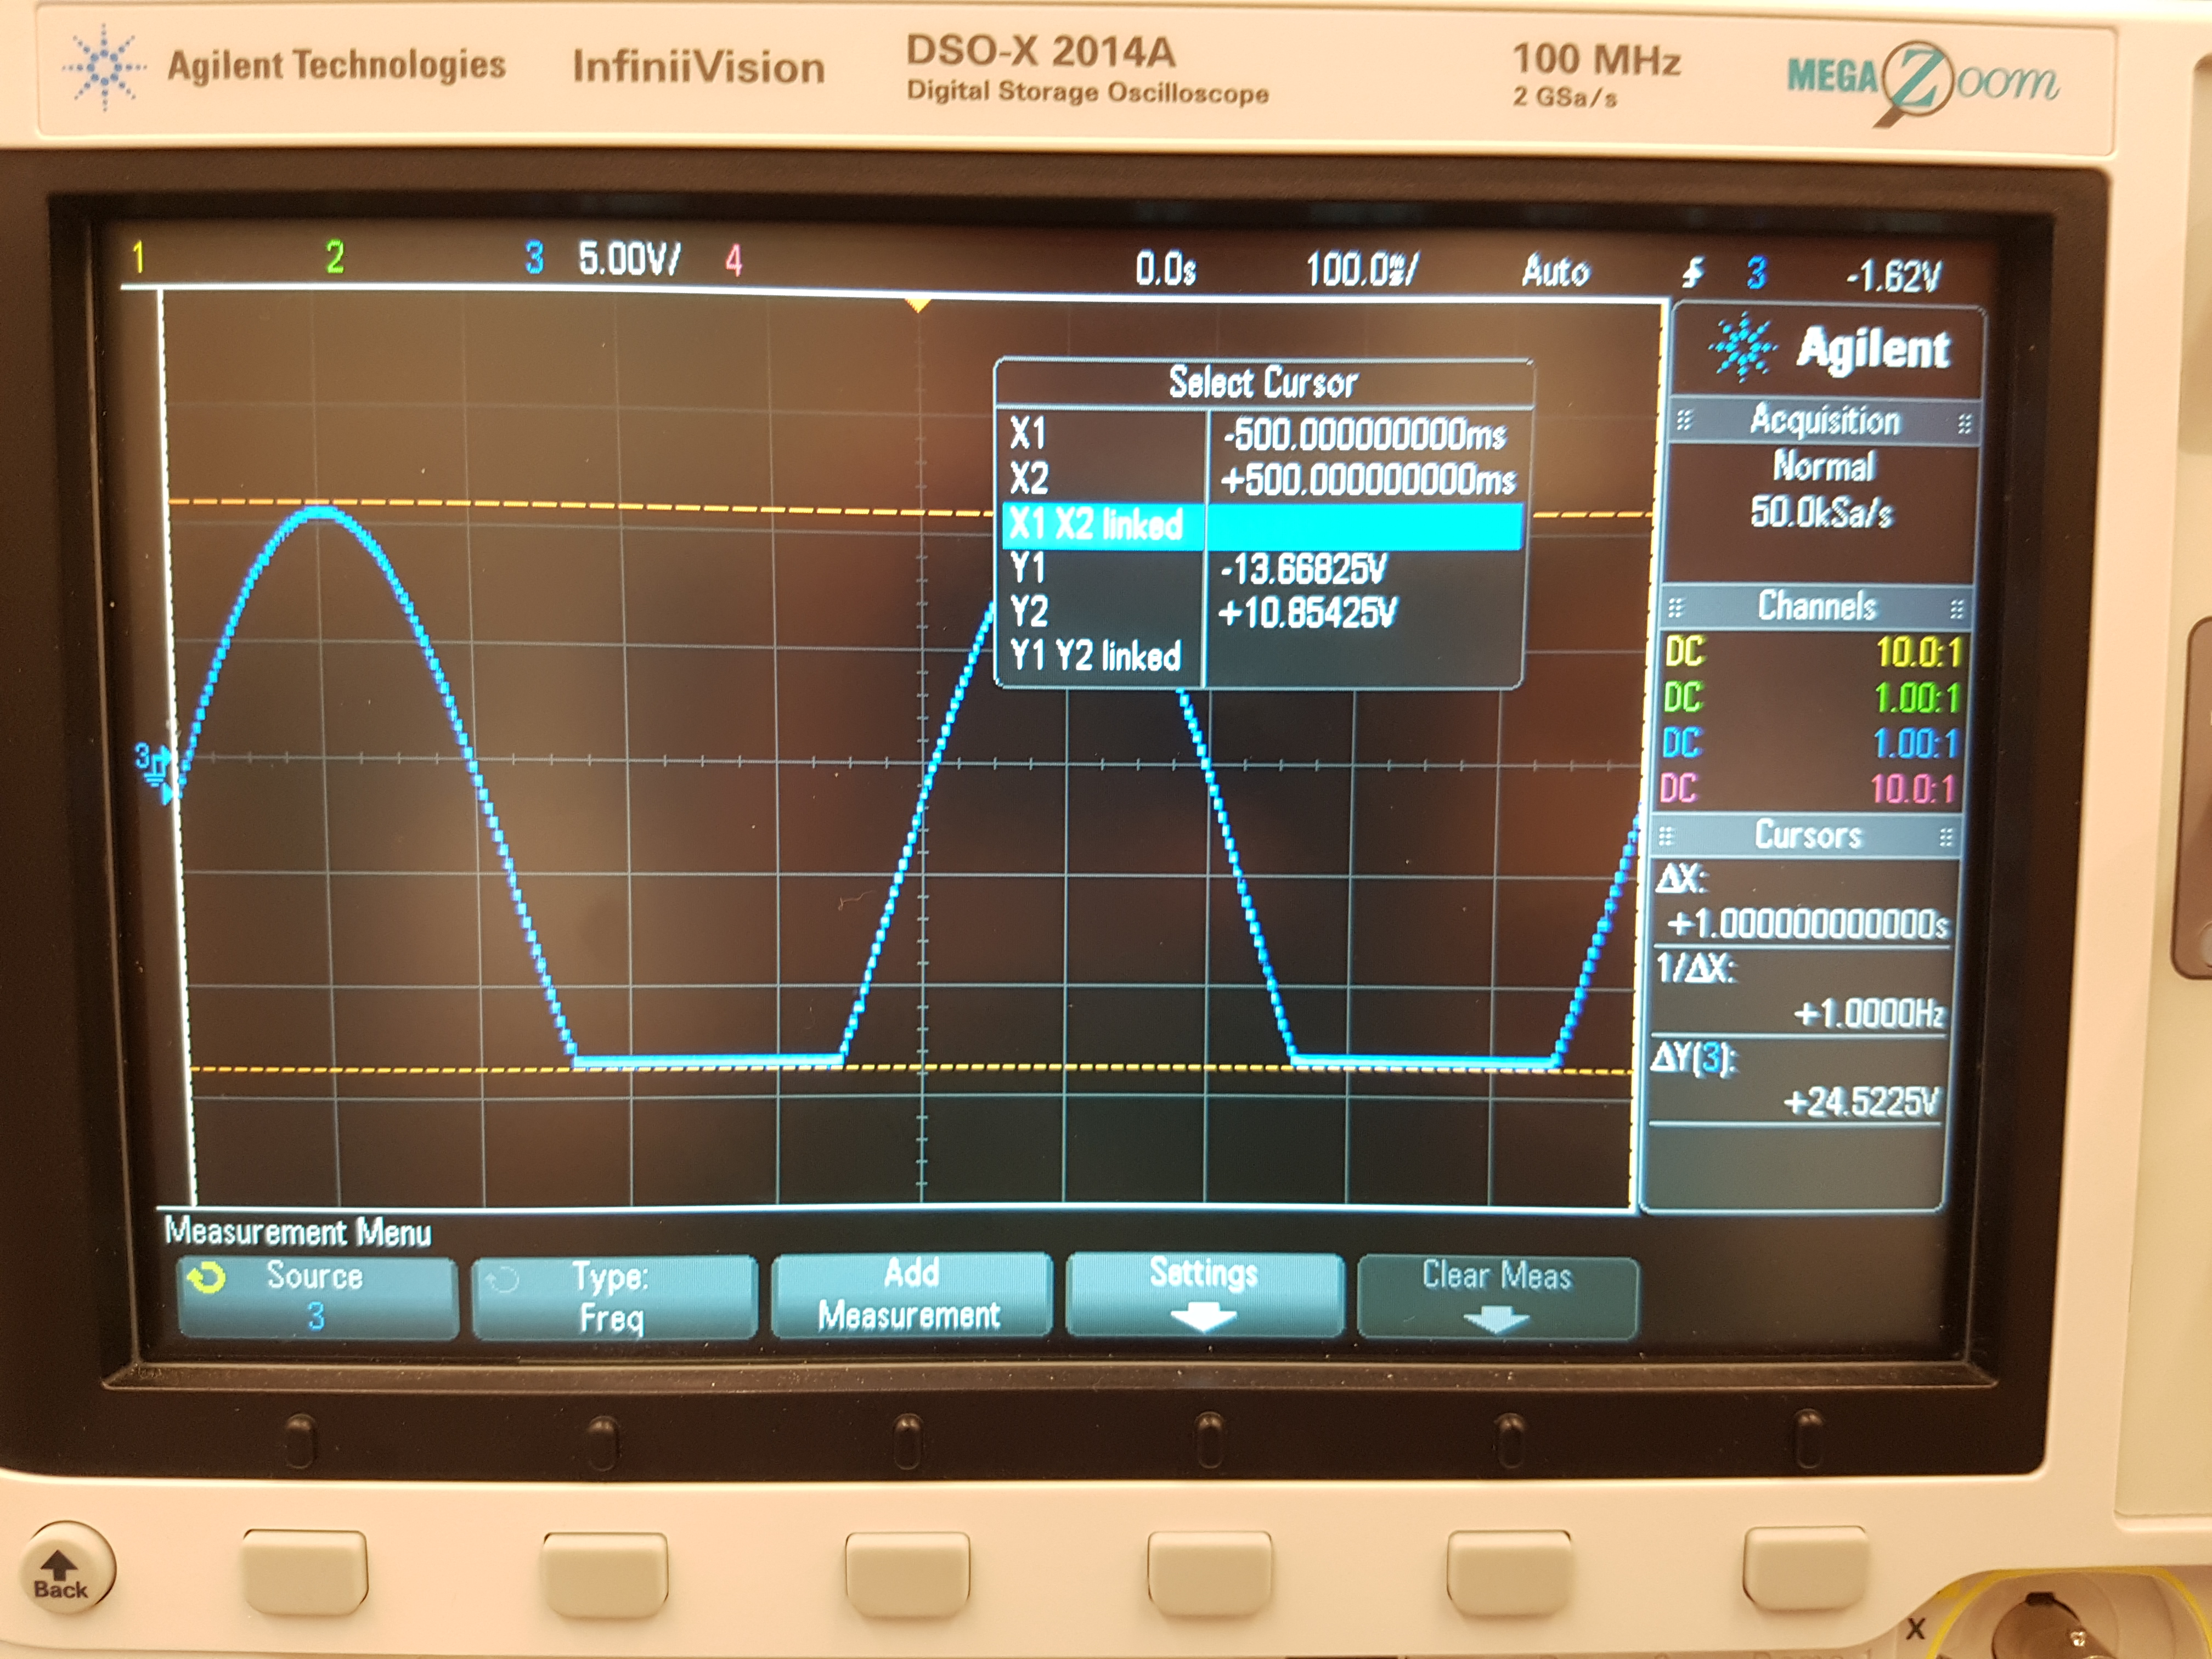
\includegraphics[scale=0.1]{osc_set2.jpg}
	\caption{Oscilloscope Output Screen Shot for 2 Sets of Inputs}
	\label{fig:scss}
\end{figure}
For the set $2$ output shown in oscilloscope, we see a flat which may come from the inappropriate y axis range setting of oscilloscope.
\subsection*{(h)}
The screen shot for beating signal we get is shown below:
\begin{figure}[H]
	\centering
	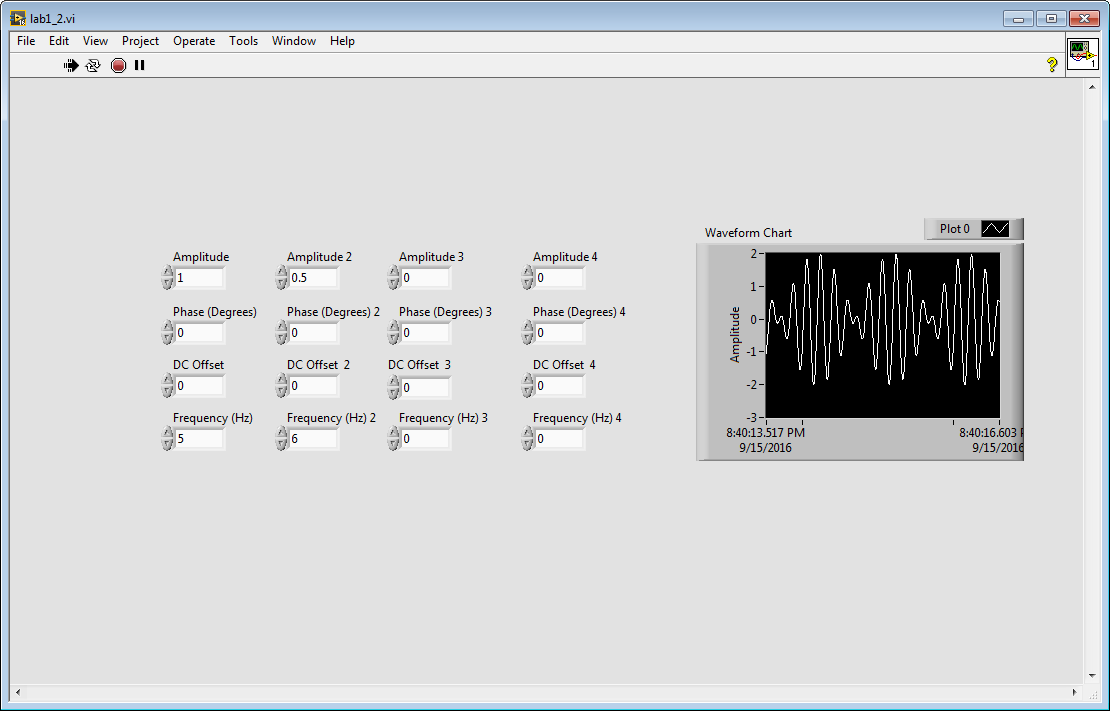
\includegraphics[scale=0.6]{beating.PNG}
	\caption{Beating Signal}
	\label{fig:beating}
\end{figure}
The beating signal is formed by making the amplitude of a sine wave varying sinusoidally. We have following methods to derive a beating signal:
$$\cos(\omega_at)\cos(\omega_bt) = \mf{\sin(\omega_at - \omega_bt + \mf{\pi}{2}) - \sin(\omega_at + \omega_bt + \mf{\pi}{2})}{2}$$, so now we can use the summation series of sine waves to form a beating signal. We choose first two signal to form it, since the gain of first two signal is $1$ and $2$ respectively in the formula, we can set the overlapping gain in Labview to $1$ and $0.5$ respectively to make two sine waves have the same overall gain equal to $1$. Then, we can set $f_1 = 5 Hz$ and $f_2 = 6 Hz$, that is $\omega_a = 11\pi$ and $\omega_b = 1\pi$, which will satisfy the conditions to form a beating signal, which is shown above.

\hspace*{3 em}
\section*{Question 3}
\subsection*{(a)}
Before powering, measure the actual voltage of the power supply and the resistance value as shown below:
$$V_s = 15.00V,\;  R_1 = 9.83K\Omega,\; R_2=9.85 K\Omega$$
Now, calculate the theoretically expected voltage output:
$$V_{out}= 15\times \mf{9.85}{9.83+9.85}=7.5076 V$$
Then, power the circuit, the actual result measured by multimeter is $V_{measure}=7.50 V$.
Though the discrepancy is not very obvious, there are still some reasons that may cause this result. First, it may be caused by the accuracy of the multimeter since it can only measure down to $0.01V$. Another possible explanation is that the handheld multimeter has internal resistance $R_m$ (loading effect), so that when we measure the voltage between a resistance, we parallel connected another resistance $R_m$ with $R_2$ as shown below.
The equivalent circuit is shown below:
\begin{figure}[H]
	\centering
	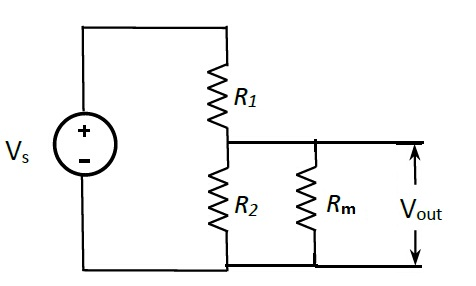
\includegraphics[scale=1.0]{q3circuit.png}
	\caption{Loading Effect Voltage Divider Circuit}
	\label{fig:load}
\end{figure}
In that case, the voltage between $R_2$ will decrease a little bit. Usually, the value of the internal resistance $R_m$ is way larger than $10K\Omega$, so the difference between theoretical value and actual value is not large here. Last but not the least, $R_1$, $R_2$ and $V_s$ are all measured by the handheld multimeter, If we count in the internal resistance when measuring , the measurement itself may not be exact accurate. Now, repeat the above experiment for ideal value $R_1=R_2=100 K\Omega$.
The actual value is shown below:
voltage input $V_s = 15.00V$,  $R_1 = 96.7K\Omega$,$R_2=98.4 K\Omega$.
The theoretically expected voltage output is:
$$V_{out}= 15\times \mf{98.4}{96.7+98.4}=7.5654 V$$
Then, power the circuit, the actual result measured by multimeter is $$V_{measure}=7.52 V$$.
The season of the discrepancy remains the same as the case above. Now, repeat the above experiment for ideal value $R_1=R_2=1 M\Omega$.
The actual value is shown below:
voltage input $V_s = 15.00V$,  $R_1 = 0.990M\Omega$, $R_2=0.989 M\Omega$.
The theoretically expected voltage output is:
$$V_{out}= 15\times \frac{0.989}{0.990+0.989}=7.4962 V$$
Then, power the circuit, the actual result measured by multimeter is $V_{measure}=7.11 V$.
This time, the discrepancy is more obvious, mainly because we parallel connected the internal resistance of multimeter $R_m$ with $R_2$.
\subsection*{(b)}
Now deduce the expression of $V_{measure}$ with the internal resistance counted in.
$$V_{measure}=15\times\frac{R_2//R_m}{R_1+R_2//R_m}$$
$$R_2//R_m=\frac{1}{\frac{1}{R_2}+\frac{1}{R_m}}=\frac{R_2R_m}{R_2+R_m}$$
$$V_{measure}=15\times\frac{\frac{R_2R_m}{R_2+R_m}}{\frac{R_2R_m+R_1R_2+R_1R_m}{R_2+R_m}}=\frac{15R_2R_m}{R_2R_m+R_1R_2+R_1R_m}$$
$$R_m=\frac{-R_1R_2V_{measure}}{(R_2+R_1)V_{measure}-15R_2}$$
Use the results from (a), $R_1 = 0.990 M\Omega$, $R_2=0.989 M\Omega$, $V_{measure}=7.52 V$. We have: 
$$R_m=\frac{-0.990\times 0.989 \times 7.11}{(0.989+0.990)\times 7.11-15\times 0.989}M\Omega$$
Hence, $R_m=9.11M\Omega$
\subsection*{(c)}
Repeat the above set of measurements using the NI 6230 DAQ to measure the voltage output. For $R_1 = 9.83K\Omega$, $R_2=9.85 K\Omega$, The ideal output voltage is $V_{out}=7.5076 V$, the DAQ value is $V_{DAQ}=7.5183$. For $R_1 = 96.7K\Omega$, $R_2=98.4 K\Omega$. The ideal output voltage is $V_{out}=7.5654 V$, the DAQ value is $V_{DAQ}=7.5708$. For $R_1 = 0.990M\Omega$, $R_2=0.989 M\Omega$. The ideal output voltage is $V_{out}=7.4962 V$, the DAQ value is $V_{DAQ}=7.5071$.\\
We could see that the ideal voltage and the actual measurement voltage are very similar, and the $V_{DAQ}$ value is even $0.01V$ larger than the ideal output. First, to figure out why $V_{DAQ}$ value is $0.01V$ larger, we measured the voltage of $R_1$ with the NI 6230 DAQ. It turns out that:
\begin{itemize}
	\item the voltage of $R_1$ in case $1$ is $V_1=7.4958V$;  
	\item the voltage of $R_1$ in case $2$ is $V_1=7.4439V$;
	\item the voltage of $R_1$ in case $3$ is $V_1=7.5097V$;
\end{itemize} 	
Thus, the total voltage is $15.01$ - $15.02V$ instead of $15.00V$, which explains why the $V_{DAQ}$ value is $0.01V$ larger than we expected.
Now, since we know that $V_{DAQ}$ is almost ideal, it means that the internal resistance of NI 6230 DAQ is much larger than $1 M\Omega$ and can be set equal to infinity in this case. The reason that NI 6230 DAQ has such a large internal resistance is because that NI 6230 DAQ uses different electrical circuit to measure the signal. NI 6230 DAQ is equipped with a module with more C-MOS Field Effect Transistor than the normal bipolar transistor used in the multimeter. Thus, after integrate several C-MOS Transistor into a single chip, the input resistance could reach to approximately infinity. This explains why the NI 6230 DAQ has such ideal accuracy.
\end{document}